\setchapterpreamble[u]{\margintoc}
\setchapterstyle{kao}

\chapter{Neutrinos in the Standard Model}

\labch{stdmodel}

The Standard Model (SM) of particle physics is a relativistic quantum field theory based on the gauge symmetry group $\mathrm{SU}(3)_C \times \mathrm{SU}(2)_L \times \mathrm{U}(1)_Y$, where the sub-scripts $C$, $L$ and $Y$ correspond to the conserved quantities \emph{color}, \emph{left-handed chirality} and \emph{weak hypercharge}, respectively. In this model, all matter particles are described as fermions, that is, excitations of Dirac-type fermion fields permeating space-time. The forces acting between fermions are mediated by an exchange of bosons, and all interactions must preserve the over-all symmetry of the theory. Since its completion in the early 1970s, it has been shown to an impressive degree of precision that it accurately describes the interactions between elementary particles due to the Strong Force, the Weak Force and the electromagnetic force. It can also explain how quarks and leptons acquire their masses via the Higgs mechanism, whose by-product, the Higgs boson, was detected at the LHC in 2012\cite{Aad_2012}. Despite its success, the Standard Model has some known shortcomings such as its incompatibility with General Relativity and inability to explain cosmological phenomena most commonly interpreted as Dark Matter and Dark Energy.  Most relevantly for this work, it predicts that neutrinos should be massless and therefore does not allow for neutrino oscillations. Since neutrino oscillations can be experimentally observed at very high statistical significance\cite{PhysRevLett.81.1562}, it is clear that the SM has to be extended in such a way that neutrino masses can be accommodated. There are several candidate theories for such an extension, but none of them could so far be confirmed experimentally. This chapter describes the properties and interactions of neutrinos as they are described by the SM. It also briefly outlines the Higgs mechanism and how it can be extended to produce neutrino masses via the introduction of right-handed "sterile" neutrino states.

\section{Standard Model particles}

The elementary particles of the SM are organized into fermions and bosons, where fermions make up the observable matter while bosons are the particles that mediate forces. The number of force-mediating bosons is determined by the generators of the symmetry groups that all interactions must obey, while the strength of each force is determined by a \emph{coupling constant} that has to be estimated experimentally. There are eight massless gluons that correspond to the generators of the $\mathrm{SU}(3)_C$ group and mediate the Strong force. All Strong interactions conserve the so-called \emph{color} charge of the involved particles. The symmetry group $\mathrm{SU}(2)_L \times \mathrm{U}(1)_Y$ is the combined symmetry of the \emph{electroweak} force and produces the gauge boson fields $W_1$, $W_2$, $W_3$ and $B$. The electroweak symmetry group is broken into the $\mathrm{U}(1)_Q$ group by interactions of fermions with the Higgs field (further described below) that mixes the $W$ and $B$ fields into massive $W^\pm$ and $Z^0$ bosons and a massless photon $\gamma$ such that
\begin{align}
    Z &= \cos \theta_W W_3 - \sin \theta_W B \\
    \gamma &= \sin \theta_W W_3 + \cos \theta_W B\\
    W^\pm &= \frac{1}{\sqrt{2}} (W_1 \mp iW_2)\;,\label{eq:ew-boson-definitions}
\end{align}
where $\theta_W$ is the so-called \emph{Weinberg angle}.
\begin{margintable}
    \caption{Fermions in the Standard Model. The electric charge, Q, is the conserved charge of the $\mathrm{U}(1)_Q$ symmetry group.}
    \label{tab:fermions-sm}
    \centering
    \begin{tabular}{ccccc} \toprule
    & \multicolumn{3}{c}{generation} & \\ \cmidrule{2-4}
    & 1 & 2 & 3 & Q \\ \midrule
    \multirow{4}{*}{\rotatebox[origin=c]{90}{quarks}}\\
    & u & c & t & $+\nicefrac{2}{3}$ \\
    & d & s & b & $-\nicefrac{1}{3}$ \\
    \\ \midrule
    \multirow{4}{*}{\rotatebox[origin=c]{90}{leptons}}\\
    & $\nu_e$ & $\nu_\mu$ & $\nu_\tau$ & 0 \\
    & $e$ & $\mu$ & $\tau$ & $-1$ \\
    \\ \bottomrule
    \end{tabular}
\end{margintable}
The fermions of the SM are divided into quarks and leptons. Quarks participate in all strong, weak and electromagnetic interactions and are always found in combinations that form baryons (protons, neutrons) or mesons (kaons, pions). The leptons, on the other hand, do not participate in strong interactions. Charged leptons are massive and participate in both the weak and the electromagnetic force, while neutral leptons, the neutrinos, are massless and participate only in weak interactions. All fermions can be grouped into three \emph{generations} of quarks and leptons that are only distinguished by their masses, leading to a convenient arrangement of quarks and leptons into a $3\times4$ scheme as shown in \reftab{fermions-sm}. For each (massive) fermion, there exists a left-handed and a right-handed component. The left-handed components of each generation form a doublet of the $\mathrm{SU}(2)_L$ group with weak isospin $\frac{1}{2}$, while the right-handed components are singlets. The right-handed and left-handed fields for one generation and their charges are summarized in \reftab{fermions-one-generation}.
\begin{margintable}
    \caption{Eigenvalues of the weak isospin $I$, of its third component $I_3$ and the hypercharge $Y = 2(Q - I_3)$ for one generation of fermions. Reproduced from \cite{giunti-kim-neutrino}.}
    \label{tab:fermions-one-generation}
    \centering
    \begin{tabular}{cccc} \toprule
    & $I$ & $I_3$ & $Y$ \\ \midrule
    \multirow{2}{*}{$L_L \equiv \begin{pmatrix} \nu_{eL} \\ e_L \end{pmatrix}$} & \multirow{2}{*}{$\nicefrac{1}{2}$} & $\nicefrac{1}{2}$ & \multirow{2}{*}{-1}\\
    & & $-\nicefrac{1}{2}$ & \\ \midrule
    $e_R$ & 0 & 0 & -2 \\ \midrule
    \multirow{2}{*}{$Q_L \equiv \begin{pmatrix} u_L \\ d_L \end{pmatrix}$} & \multirow{2}{*}{$\nicefrac{1}{2}$} & $\nicefrac{1}{2}$ & \multirow{2}{*}{$\nicefrac{1}{3}$}\\
    & & $-\nicefrac{1}{2}$ & \\ \midrule
    $u_R$ & 0 & 0 & $\nicefrac{4}{3}$ \\
    $d_R$ & 0 & 0 & $-\nicefrac{2}{3}$ \\\bottomrule
    \end{tabular}
\end{margintable}

\subsection{Spin, Helicity and Chirality}
The states that describe fundamental particles must, by definition, belong to irreducible representations of the Poincar\'{e} group. All possible representations can be classified so-called Casimir operators, which are operators that are invariant under the group transformations. The first Casimir operator for the Poincar\'{e} group is the square of the four-momentum
\begin{equation}
    P^2 = P_\mu P^\mu
\end{equation}
with the eigenvalue $p^2 = m^2$ being the rest-mass of the particle. The second one is the square of the so-called Pauli-Lubanski four-vector
\begin{equation}
    W^2 = W_\mu W^\mu = -m^2 \vec{S}^2\;,
\end{equation}
which has the eigenvalue $w^2 = -m^2 s(s+1)$, where $s$ is the spin of the particle. Thus, all representations of the Poincar\'{e} group can be classified by their rest mass and spin. Given $m$ and $s$ for a particle, different states of that particle can be distinguished by their momentum $\vec{p}$ and the zeroth component of $W^\mu$, which is $W^0 = \vec{S}\vec{p}$. A convenient quantum number to define is the \emph{helicity} of a particle, which is the eigenvalue of the operator
\begin{equation}
    \hat{h} = \frac{\vec{S}\vec{p}}{s |\vec{p}|}
\end{equation}
that can have values of $\pm1$. The relativistic properties of a particle with known mass and spin are fully described by a measurement of its momentum, $\vec{p}$, and helicity, $h$.

The states of spin-$\nicefrac{1}{2}$ fermions, such as neutrinos, are representations of the Poincar\'{e} group that are constructed out of two spinors, $\Psi_L$ and $\Psi_R$, that are called \emph{left-handed} and \emph{right-handed}, respectively. Their propagation is governed by the Dirac equation, which reads in Fourier space
\begin{equation}
\begin{aligned}
    (E - \vec{\sigma}\cdot \vec{p})\Psi_R &= m \Psi_L \\
    (E + \vec{\sigma}\cdot \vec{p})\Psi_L &= m \Psi_R
\end{aligned}\;.\label{eq:dirac-chirality}
\end{equation}
Whether a particle is left-handed or right-handed is referred to as its \emph{chirality}. If the mass in \refeq{dirac-chirality} is zero, the two fields describe independent particles that are eigenstates of the helicity operator, which is $\hat{h}=\frac{\vec{\sigma}\vec{p}}{|\vec{p}|}$ in this case. This means that helicity and chirality eigenstates are identical for massless particles, but for massive particles, helicity eigenstates are superpositions of $\Psi_L$ and $\Psi_R$.

\subsection{Electroweak Symmetry Breaking}
\labsec{ew-symmetry-breaking}
The process of breaking the $\mathrm{SU}(2)_L \times \mathrm{U}(1)_Y$ symmetry group deserves special attention for the purposes of this work, because it is the process by which the exchange bosons of the Weak force acquire their mass. If the symmetry was unbroken, as it is the case for the $\mathrm{SU(3)}$ group of the Strong force, then the exchange bosons would all remain massless, just like the gluons. To simplify the discussion, the process can be illustrated using only the first generation of SM fermions. The starting point is to introduce the Higgs doublet of complex scalar fields
\begin{equation}
    \Phi = \begin{pmatrix}
        \Phi^+ \\
        \Phi^0
    \end{pmatrix}\;,\label{eq:higgs-doublet}
\end{equation}
where $\Phi^+$ is charged and $\Phi^0$ is neutral\sidenote{In a more general discussion, the Higgs doublet would be written down without assigning the charges a priori, they would be derived later. See \cite{schwartz_2013} for a more rigorous derivation.}. The Lagrangian describing the dynamics of this field,
\begin{equation}
    \mathcal{L}_\mathrm{Higgs} = (D_\mu \Phi^\dag)(D^\mu \Phi) - \lambda \left( \Phi^\dag \Phi - \frac{v^2}{2} \right)^2\;,\label{eq:higgs-lagrangian}
\end{equation}
with the covariant derivative
\begin{equation}
    D_\mu \Phi= \partial_\mu \Phi - ig W_\mu^a \tau^a \Phi - \frac{1}{2}ig'B_\mu \Phi
\end{equation}
is invariant under $\mathrm{SU}(2)_L \times \mathrm{U}(1)_Y$ symmetry and adds a quartic self-interaction potential with the parameters $\lambda$ and $v$, where $\lambda$ is taken to be positive, such that the potential is bounded from below. The fields $W_\mu^a$ in the covariant derivative correspond to the gauge bosons of the $\mathrm{SU}(2)_L$ group whose generators are $\tau^a = \frac{\sigma^a}{2}$, where $\sigma^a$ are the Pauli matrices. The $B_\mu$ field is the boson of the $\mathrm{U}(1)_Y$ group. The factors $g$ and $g'$ are the $\mathrm{SU}(2)_L$ and $\mathrm{U}(1)_Y$ coupling constants, respectively, and are related to the Weinberg angle by
\begin{equation}
    \tan \theta_W = \frac{g'}{g}\;.\label{eq:weinberg-angle}
\end{equation}
Because the potential has a minimum that is not at zero, the field $\Phi$ acquires a non-zero \emph{vacuum expectation value} (VEV) where $\Phi^\dag \Phi = \frac{v^2}{2}$. Since the vacuum is electrically neutral, this VEV can only come from the neutral part, $\Phi^0$, of the doublet and can be written as
\begin{equation}
    \Phi_\mathrm{VEV} = \frac{1}{\sqrt{2}}\begin{pmatrix}
        0\\
        v
    \end{pmatrix}\;.
\end{equation}
This vacuum expectation value is no longer symmetric under the $\mathrm{SU}(2)_L \times \mathrm{U}(1)_Y$ group, but it still is symmetric under the $\mathrm{U}(1)_Q$ group in which electric charge is conserved. To see what happens to the Lagrangian, the field $\Phi$ can be expressed in the unitary gauge as a variation around the VEV such that
\begin{equation}
    \Phi(x) = \frac{1}{\sqrt{2}}\begin{pmatrix}
        0 \\
        v + H(x)
    \end{pmatrix}\;.
\end{equation}
Plugging this into the Lagrangian in \refeq{higgs-lagrangian} and re-writing the $W_\mu^i$ and $B_\mu$ fields in terms of $Z$ and $W^\pm$ using the relationships given in \refeq{ew-boson-definitions} and \refeq{weinberg-angle} we find
\begin{equation}
\begin{aligned}
    \mathcal{L}_\mathrm{Higgs} = &\hspace{1em}\frac{1}{2}(\partial H)^2 - \lambda v^2 H^2 - \lambda v H^3 - \frac{\lambda}{4}H^4 \\
    &+ \frac{g^2v^2}{4} W_\mu^\dag W^\mu + \frac{g^2 v^2}{8\cos^2\theta_W}Z_\mu Z^\mu \\
    &+ \mathrm{Higgs\;vertices}\;,
    \label{eq:boson-mass-terms}
\end{aligned}
\end{equation}
where Higgs vertices are 3-vertices and 4-vertices between the Higgs field and the $W$ and $Z$. The notable part is that the $W$ and $Z$ bosons have acquired a kinetic term in the second line of \refeq{boson-mass-terms} with a mass that is proportional to the VEV of the Higgs field, giving massive exchange bosons to the Weak force\sidenote{The massless photon field is found by expanding the full electroweak Lagrangian in the same way, which we neglect here for the sake of brevity.}.

\subsection{Charged Fermion Masses}
\label{sec:charged-fermion-masses}
In Quantum Electrodynamics, a Lorentz-invariant mass term for spin-$\frac{1}{2}$ fermions can be written as a product of left-handed and right-handed Weyl spinors, also known as the Dirac mass
\begin{equation}
    \mathcal{L}_\mathrm{Dirac} = m (\bar{\Psi}_R \Psi_L - \bar{\Psi}_L \Psi_R)\;.
\end{equation}
However, such a term is not invariant under $\mathrm{SU}(2)_L \times \mathrm{U}(1)_Y$ and therefore cannot be added to the SM Lagrangian directly. Fortunately, masses for fermions can be recovered if we add a Yukawa coupling term between the fermions and the Higgs field, such as
\begin{equation}
    \mathcal{L}_\mathrm{Yuk} = -y \bar{L}_L \Phi e_R + \mathrm{h.c.}\;,
\end{equation}
where $L_L$ denotes the $\mathrm{SU}(2)_L$ doublet listed in \reftab{fermions-one-generation} and $y$ is the Yukawa coupling constant. When the VEV is inserted into this term, it produces a mass term $-m_e (\bar{e}_L e_R + \bar{e}_R e_L)$ with $m_e = \frac{y}{\sqrt{2}}v$ for the charged leptons and the down-type quarks $d$, $s$, and $b$.  A similar term that is also invariant under $\mathrm{SU}(2)_L$ and generates masses for the up-type quarks is $-y \bar{L}_L \tilde{\Phi} u_R$, where we defined $\tilde{\Phi} \equiv i \sigma_2 \Phi$. When all possible terms of this form for all generations of quarks are put together, the generations mix among each other in a way that is very similar to neutrino mixing.

\subsection{Neutrino Masses}
\labsec{neutrino-masses}
The Higgs mechanism described in \refsec{charged-fermion-masses} necessitates both left-handed and right-handed Weyl spinors to interact with the Higgs field. Since there are no right-handed neutrinos in the SM, it predicts that they should be massless, in contradiction to experimental evidence. However, if we add right-handed neutrino fields into the model, then neutrino masses can be generated in a way that is tantalizingly similar to that of up-type quarks by adding interactions of the form $Y_{ij}^\nu \bar{L}^i \tilde{\Phi}\nu_R^j$ to the Lagrangian. Such a right-handed field would be uncharged with respect to all symmetry groups of the SM and would therefore not interact with any other particle and is hence referred to as a \emph{sterile neutrino}. Because neutrinos are electrically neutral, another possibility for a mass term that is allowed by the symmetry of the SM is the so-called \emph{Majorana mass}, $m \nu_R^c \nu_R$, in which $\nu_R^c=\nu_R^T \sigma_2$ is the charge conjugate Weyl spinor.

\subsubsection{Dirac Mass}

Dirac masses are produced by adding Yukawa couplings
\begin{equation}
    \mathcal{L}_\mathrm{Yuk} = -Y_{ij}^e \bar{L}^i \Phi e_R^j - Y_{ij}^\nu \bar{L}^i \tilde{\Phi} \nu_R^j + \mathrm{h.c.}
\end{equation}
to the Lagrangian, where the indices $i$ and $j$ run over the generations $e$, $\mu$, and $\tau$ and the matrices $Y_{e,\nu}$ contain the complex Yukawa coupling constants that are free parameters of the model. After symmetry breaking, the mass terms become
\begin{equation}
\begin{aligned}
  \mathcal{L}_\mathrm{mass} &= -\frac{v}{\sqrt{2}}\left[  Y^e_{ij} \bar{e}_L^i e_R^j +  Y^\nu_{ij} \bar{\nu}_L^i \nu_R^j \right] + \mathrm{h.c.} \\
  &=  -\frac{v}{\sqrt{2}}\left[ \bar{e}_L Y_e e_R + \bar{\nu}_L Y_\nu \nu_R \right] + \mathrm{h.c.}\;.
\end{aligned}
\end{equation}
To find the physical fields with definite masses, the $Y_{e,\nu}$ matrices are diagonalized with two unitary matrices
\begin{align}
    Y_e &= U_e M_e K_e^\dag &Y_\nu &= U_\nu M_\nu K_\nu^\dag\;,
\end{align}
such that $M_{e,\nu}$ are diagonal and contain the physical masses of leptons and neutrinos. By applying the transformation
\begin{equation}
\begin{aligned}
    e_L &\rightarrow U_e e_L, &e_R &\rightarrow K_e e_R \\
    \nu_L &\rightarrow U_\nu \nu_L, &\nu_R &\rightarrow K_\nu \nu_R\;, \label{eq:mass-basis-trafo}
\end{aligned}
\end{equation}
the Lagrangian can be written in the \emph{mass basis}
\begin{equation}
    \mathcal{L}_\mathrm{mass} = \frac{v}{\sqrt{2}} \left[ \bar{e}_L M_e e_R - \bar{\nu}_L M_\nu \nu_R \right]\;.\label{eq:mass-lagrangian-diagonal}
\end{equation}
Applying these transformations to the lepton fields will also affect the interaction part of the electroweak Lagrangian for leptons, but not all of them are of any physical consequence. Since there is no coupling to right-handed neutrinos, the transformation of $\nu_R$ has no effect at all and we can simply ignore $K_\nu$. The transformation of the right-handed charged leptons enters the coupling term to the $B$ gauge boson, but it exactly cancels since $K^\dag K = \mathbb{1}$. The transformations $e_L \rightarrow U_e e_L$ and $\nu_L \rightarrow U_\nu \nu_L$ on their own enter the coupling to the combined $B$ and $W_3$ bosons (which become the $Z$ boson after symmetry breaking), but they also cancel because neutral-current interactions do not mix neutrinos and charged leptons\sidenote{This cancellation is also known as the GIM mechanism.}. The only physically relevant effect is on the charged-current interactions for which the Lagrangian in the mass basis becomes
\begin{equation}
    \mathcal{L}_\mathrm{CC,\;mass\;basis} = \frac{g}{\sqrt{2}}
    \left[
        W^+_\mu \bar{\nu}_L^i \gamma^\mu (U)^{ij} e_L^j
        + W^-_\mu \bar{e}_L^i \gamma^\mu (U^\dag)^{ij} \nu_L^j
    \right],\label{eq:lag-cc-mass-basis}
\end{equation}
where $U\equiv U_\nu^\dag U_e$ is the PNMS matrix, which is analogous to the CKM matrix in the quark sector. In general, $U$ is a complex unitary matrix that can be parametrized by three real angles and six phases. However, most of the phases can be set to zero by globally rotating the complex phases of the fields without changing the Lagrangian. Only one phase remains that cannot be cancelled this way, which is referred to as the \emph{Dirac phase}, leaving four real degrees of freedom in $U$. A Dirac phase different from zero leads to CP violation.
As a consequence of the mixing between generations in \refeq{lag-cc-mass-basis}, charged-current weak interactions that produce a neutrino always generate a superposition of mass eigenstates, which leads to neutrino oscillations. If we define neutrino \emph{flavor eigenstates} as
\begin{equation}
    \begin{pmatrix}
        \nu_{L}^e \\
        \nu_{L}^\mu \\
        \nu_{L}^\tau
    \end{pmatrix}
    = U^\dag
    \begin{pmatrix}
        \nu_{L}^1 \\
        \nu_{L}^2 \\
        \nu_{L}^3
    \end{pmatrix}\;,
\end{equation}
then the Lagrangian in \refeq{lag-cc-mass-basis} can be written in the \emph{flavor basis} as in \refeq{ew-cc-lagrangian}. The flavor states of the charged leptons are identical to their mass eigenstates and therefore do not mix among each other. It is worth noting that, in this picture of pure Dirac neutrino masses, there is no mixing between the left-handed and the right-handed states, and therefore there is no observable oscillation effect that could be measured between active and sterile neutrinos.

\subsubsection{Dirac-Majorana Masses}

There exists another term that can generate fermion masses that does not require an interaction between left-handed and right-handed spinors that was discovered by E. Majorana. If $\Psi_L$ is a left-handed chiral Weyl spinor, then the term
\begin{equation}
   m \Psi_L^T \mathcal{C}^\dag \Psi_L = m \Psi_L^c \Psi_L
\end{equation}
is a Lorentz-invariant mass term, in which $\mathcal{C}$ is the charge conjugation operator. The reason why this term cannot be used to give masses to all the fermions in the SM is that it is not invariant under any of the SM symmetries. However, if we propose that right-handed neutrinos exist and that they are singlets under all SM symmetries, then a Majorana mass term can be added for them without breaking the global SM symmetry. The most general Lagrangian including all Yukawa couplings and Majorana mass terms (excluding left-handed neutrino majorana masses) of the lepton sector is
\begin{equation}
  \mathcal{L}_\mathrm{mass} = -Y_{ij}^e \bar{L}^i \Phi e_R^j - Y_{ij}^\nu \bar{L}^i \tilde{\Phi} \nu_R^j - \frac{1}{2}M_{kl}(\nu_R^k)^c \nu_R^l + \mathrm{h.c.}\;,
\end{equation}
where the indices $i$ and $j$ run over the generations $e$, $\mu$, and $\tau$ and the matrix $Y_{ij}^e$ contains the Yukawa coupling constants, while the matrix $M_{kl}$ contains the Majorana masses with the indices $k$ and $l$ running over the $N_s$ sterile states $s_1$ to $s_{N_s}$. While it seems natural to associate exactly one sterile right-handed state with each active flavor, the model does in principle allow for any number $N_s$ of sterile neutrinos. By placing all the left-handed and charge-conjugated right-handed fields in column vectors
\begin{equation}
\begin{aligned}
  \boldsymbol{N}_L &= \begin{pmatrix} \boldsymbol{\nu}_L \\ \boldsymbol{\nu}_R^c \end{pmatrix}
  &\boldsymbol{\nu}_R^c  &= \begin{pmatrix}\nu_{s_{1} R}^c \\ \vdots \\ \nu_{s_{N_{s}} R}^c\end{pmatrix}
\end{aligned}
\end{equation}
the Dirac and Majorana mass terms that are produced after symmetry breaking can be written in a unified notation as
\begin{equation}
  \mathcal{L}_\mathrm{mass}^\mathrm{D+M} = \frac{1}{2} \boldsymbol{N}_L^T \mathcal{C}^\dag M^\mathrm{D+M} \boldsymbol{N}_L + h.c.
\end{equation}
with the symmetric mass matrix
\begin{equation}
  M^\mathrm{D+M} \equiv
  \begin{pmatrix}
  0 & (M^D)^T \\
  M^D & M^R
  \end{pmatrix}\;.\label{eq:dm-mass-matrix}
\end{equation}
The mass eigenstates are linear combinations of states that linearize the mass matrix in \refeq{dm-mass-matrix}. In contrast to the pure Dirac mass, this linear combination allows for mixing between active and sterile states, and therefore oscillation effects such as those that are tested in this work are possible. Another consequence of this mixing is that the GIM mechanism no longer works, because the part of the mixing matrix applying to active flavors is no longer unitary. It is therefore possible for transitions between different mass eigenstates to occur in neutral-current interactions, which can lead to the production of Heavy Neutral Leptons (HNL)\todo{add paper citation?}.

\subsection{See-Saw Mechanism}

One of the puzzles of the SM is the question of why the neutrino masses are much smaller than those of the other fermions. If neutrino masses are purely Dirac, then the masses are proportional to the VEV of the Higgs field and their Yukawa couplings as can be seen in \refeq{lag-cc-mass-basis}. For neutrino masses to be small, the couplings would have to be fine tuned to be very small. If, on the other hand, neutrino masses are the result of combined Dirac-Majorana masses, then the mass of the active neutrino flavors is suppressed if the mass of the right-handed neutrinos is large. This can be understood very simply if we look at the mass term for only one generation where the mass matrix in \refeq{dm-mass-matrix} is a $2\times2$ matrix with a Dirac mass $m_D$ in the off-diagonal entries and a Majorana mass, $M$, in the lower right corner. The physical masses, that is, the eigenvalues of the mass matrix, are
\begin{equation}
    m_{1,2} = \sqrt{m_D^2 + \frac{1}{4}M^2} \pm \frac{1}{2} M\;.
\end{equation}
In the limit where $M \gg m_D$, the two solutions are approximately $m_\mathrm{heavy} \approx M$ and $m_\mathrm{light} \approx \frac{m_D^2}{M}$. This is, in essence, the \emph{see-saw mechanism}: As $M$ goes up, the masses of the active flavors go down. The picture becomes more complicated when all three flavors are involved, but if the Majorana masses are much larger than the Dirac masses, the mass matrix can be approximately diagonalized by blocks for a similar effect.


\section{Neutrino Properties}

\subsection{Quantum Numbers}
Neutrinos in the SM are described as having a spin of $\nicefrac{1}{2}$ and exclusively left-handed chirality. Since they are massless, their helicity is also fixed to $h=-1$. Antineutrinos are conversely right-handed with a helicity of $h=1$. As evidenced by neutrino oscillations, they do have a very small mass, but so far only upper limits could be measured experimentally.

\subsection{Mass}
Due to their high abundance in the universe, neutrinos play an important role in the evolution of large structures in our cosmos in a way that is dependent on their masses. Cosmological observations and fits assuming the $\Lambda$CDM model provide the most stringent limit on the sum of neutrino masses at
\begin{equation}
    \sum m_i < \SI{0.12}{\eV}
\end{equation}
at 95\% C.L.\cite{Planck2018,PhysRevD.103.083533}. While these limits are very constraining, they strongly depend on the underlying cosmological assumptions.

The most sensitive direct neutrino mass measurement to date comes from the KArlsruhe TRItium Neutrino (KATRIN) experiment that measures the energy spectrum of the $\beta$-decay of molecular tritium
\begin{equation}
    T_2 \rightarrow \mathrm{^3HeT^+} + e^- + \bar{\nu}_e\;.
\end{equation}
A non-zero mass $m_\nu$ of the neutrino reduces the maximum possible energy that the outgoing electron can carry, and therefore shifts the endpoint of the energy spectrum. As described in \refsec{neutrino-masses}, the flavor eigenstate $\nu_e$ is not a mass eigenstate, but is instead a superposition of several mass eigenstates whose observable mass can be approximated as $m^2_\nu = \sum_i |U_{ei}|^2m_i^2$, where $U$ is the PNMS matrix. The at 90\% C.L. upper bound on the neutrino mass from the latest KATRIN result\sidecite{KATRIN2022} is
\begin{equation}
    m_\nu < \SI{0.8}{\eV}\;.
\end{equation}
This limit has the benefit of being independent of assumptions about whether neutrino masses are Dirac or Majorana and of cosmological models.

\subsection{Active Neutrino Flavors}

The number of active neutrino flavors (that is, flavors that interact via the Weak force) can be constrained by measurements of the decay width of the $Z^0$ boson. A $Z^0$ can decay into hadrons, charged leptons, and neutrinos, with respective decay widths $\Gamma_h$, $\Gamma_\mathcal{l}$, and $\Gamma_\nu$. The total decay width scales with the number of active flavors, because each flavor provides an additional decay channel that increases the decay probability. Since neutrinos are invisible to the detector, the invisible part of the total decay width, $\Gamma_\mathrm{inv}$, can be attributed to decays to neutrinos and the number of active flavors is
\begin{equation}
    N_\nu = \frac{\Gamma_\mathrm{inv}}{\Gamma_\mathcal{l}}\left( \frac{\Gamma_\mathcal{l}}{\gamma_\nu} \right)_\mathrm{SM}\;,
\end{equation}
where $\Gamma_\mathcal{l} / \gamma_\nu$ is calculated from the SM. This measurement has been done at the LEP using $e^+ + e^-$ collisions at the $Z^0$ resonance energy with the result\sidecite{LEP2006}
\begin{equation}
    N_\nu = \num{2.9840 +- 0.0082}\;,
\end{equation}
which is compatible with the assumption of three active neutrino flavors. The result only constrains the number of neutrino states that are weakly interacting and that are lighter than the $Z^0$ mass, and therefore does not preclude the existence of additional sterile neutrinos.

\section{Neutrino Interactions}
\label{sec:ew-interactions}

Left-handed neutrinos and right-handed antineutrinos can interact with quarks and leptons via the exchange of $Z^0$ (neutral-current) and $W^\pm$ (charged-current) bosons.
In practice, neutrinos are observed to either scatter off of electrons in reactions such as
\begin{equation}
    \nu_e + e^- \rightarrow \nu_e + e^-\;,
\end{equation}
or to interact with nucleons.
While the calculation of electron scattering is straight-forward from the electroweak Lagrangian, the scattering off nuclei is rather complicated and requires different approximations depending on the energy scale.
This chapter first describes the scattering processes that are most important for the purpose of neutrino detection at energies of \SI{>1}{\giga\eV}, where the total cross-section is dominated by interactions with nuclei.
It then briefly summarizes the process of coherent forward scattering that influences neutrino oscillations during propagation through bulk material.

\subsection{Weak interactions after symmetry-breaking}
Neutrino interactions with matter are described by Weak force interactions after electroweak symmetry-breaking described in \refsec{ew-symmetry-breaking}.
The Lagrangian for these interactions can be written as the sum of the neutral-current (NC) and charged-current (CC) interactions.
The NC part describes the exchange of neutral $Z^0$ bosons, which couples to all quarks and leptons except for right-handed neutrinos (if they exist).
For leptons, the NC Lagrangian reads
\begin{marginfigure}
\centering
\begin{subfigure}[t]{0.49\linewidth}
    \begin{tikzpicture}
        \begin{feynman}
        \def\flen{1.2}
        \def\boslen{1.2}
        \def\fangle{45}

        % in order to get the [dot] to work, we need to add the empty braces
        \vertex (v1) [dot] at (0, \boslen) {};
        \vertex (i1) at ($(v1) + (180-\fangle:\flen)$) {\(\pbar{\nu}_\mathcal{l}\)};
        \vertex (f1) at ($(v1) + (\fangle:\flen)$) {\(\pbar{\nu}_\mathcal{l}\)};
        \vertex (v2) at (0, 0);

        \diagram* {
          (i1) -- [fermion] (v1) -- [fermion] (f1),
          (v1) -- [boson, edge label=$Z^0$] (v2)
        };
        \end{feynman}
    \end{tikzpicture}
    \caption{neutrinos}
\end{subfigure}
\begin{subfigure}[t]{0.49\linewidth}
    \begin{tikzpicture}
        \begin{feynman}
        \def\flen{1.2}
        \def\boslen{1.2}
        \def\fangle{45}

        % in order to get the [dot] to work, we need to add the empty braces
        \vertex (v1) [dot] at (0, \boslen) {};
        \vertex (i1) at ($(v1) + (180-\fangle:\flen)$) {\(\mathcal{l}^\pm\)};
        \vertex (f1) at ($(v1) + (\fangle:\flen)$) {\(\mathcal{l}^\pm\)};
        \vertex (v2) at (0, 0);

        \diagram* {
          (i1) -- [fermion] (v1) -- [fermion] (f1),
          (v1) -- [boson, edge label=$Z^0$] (v2)
        };
        \end{feynman}
    \end{tikzpicture}
    \caption{charged leptons}
\end{subfigure}
\caption{Neutral-current lepton interaction vertices.}
\label{fig:nc-vertices}
\end{marginfigure}
\begin{equation}
  \mathcal{L}_\mathrm{NC,L} = -\frac{g}{2 c_W^2} \sum_{\mathcal{l}=e,\mu,\tau} (\bar{\nu}_{\mathcal{l}, L} \gamma^\mu \nu_{\mathcal{l}, L} + (2 s_W^2 - 1) \bar{e}_{\mathcal{l}, L} \gamma^\mu e_{\mathcal{l}, L} + 2s_w^2 \bar{e}_{\mathcal{l}, R} \gamma^\mu e_{\mathcal{l}, R}) Z^0_\mu\;, \label{eq:ew-nc-lagrangian}
\end{equation}
where $\nu$ denotes a neutrino field, $e$ a lepton field and the subscripts $L$ and $R$ denote left-handed and right-handed fields, respectively.
The coefficient $s_W$ ($c_W$) is the sine (cosine) of the Weinberg angle and $g$ is the coupling constant that determines the overall strength of the electroweak force.
This Lagrangian leads to the trilinear couplings shown in \reffig{nc-vertices}.
The couplings to quarks have the same form as those to the charged leptons up to a difference in coupling strength\sidenote{Quark mixing has no effect on neutral current interactions due to the GIM mechanism.}.
Neutral-current interactions conserve both the electric charge and lepton number, such that a neutral-current interaction of a neutrino will always produce a neutrino of the same flavor.

The charged-current (CC) part of the Weak Lagrangian in the flavor basis is
\begin{marginfigure}
\centering
\begin{subfigure}[t]{0.49\linewidth}
    \begin{tikzpicture}
        \begin{feynman}
        \def\flen{1.2}
        \def\boslen{1.2}
        \def\fangle{45}

        % in order to get the [dot] to work, we need to add the empty braces
        \vertex (v1) [dot] at (0, \boslen) {};
        \vertex (i1) at ($(v1) + (180-\fangle:\flen)$) {\(\bar{\nu}_\mathcal{l}\)};
        \vertex (f1) at ($(v1) + (\fangle:\flen)$) {\(\mathcal{l}^{+}\)};
        \vertex (v2) at (0, 0);

        \diagram* {
          (i1) -- [fermion] (v1) -- [fermion] (f1),
          (v1) -- [boson, edge label=$W^-$] (v2)
        };
        \end{feynman}
    \end{tikzpicture}
    \caption{$W^-$ vertex}
\end{subfigure}
\begin{subfigure}[t]{0.49\linewidth}
    \begin{tikzpicture}
    \begin{feynman}
        \def\flen{1.2}
        \def\boslen{1.2}
        \def\fangle{45}

        % in order to get the [dot] to work, we need to add the empty braces
        \vertex (v1) [dot] at (0, \boslen) {};
        \vertex (i1) at ($(v1) + (180-\fangle:\flen)$) {\(\nu_\mathcal{l}\)};
        \vertex (f1) at ($(v1) + (\fangle:\flen)$) {\(\mathcal{l}^{-}\)};
        \vertex (v2) at (0, 0);

        \diagram* {
          (i1) -- [fermion] (v1) -- [fermion] (f1),
          (v1) -- [boson, edge label=$W^+$] (v2)
        };
    \end{feynman}
    \end{tikzpicture}
    \caption{$W^+$ vertex}
\end{subfigure}
\caption{Charged-current lepton interaction vertices.}
\label{fig:cc-vertices}
\end{marginfigure}
\begin{equation}
    \mathcal{L}_\mathrm{CC} = -\frac{g}{\sqrt{2}} \sum_{\mathcal{l}=e,\mu,\tau} \bar{\nu}_{\mathcal{l},L} \gamma^\mu e_{\mathcal{l},L} W^+_\mu + \bar{e}_{\mathcal{l},L} \gamma^\mu \nu_{\mathcal{l},L} W^-_\mu\;\mathrm{+h.c.}\;.\label{eq:ew-cc-lagrangian}
\end{equation}
In contrast to neutral current interactions, the charged current interactions couple exclusively to left-handed fields\sidenote{The left-handed fields in the flavor basis are superpositions of mass eigenstates that may contain a (charge-conjugated) right-handed Majorana component as described in \refsec{neutrino-masses}}.
The associated lepton interaction vertices are shown in \reffig{cc-vertices}.

The weak CC interactions with quarks are affected by quark mixing as a result of their mass generation via the Higgs mechanism.
After electroweak symmetry breaking, the mass eigenstates and the flavor eigenstates of quarks are not identical but are instead mixed with a unitary matrix, $V$, that is also called the Cabbibo-Kobayashi-Maskawa (CKM) matrix.
In the basis of mass eigenstates, the Lagrangian for weak CC interactions with quarks is
\begin{equation}
    \mathcal{L}_\mathrm{CC,Q} = \frac{g}{\sqrt{2}} \sum_{\alpha=1}^3 \sum_{\beta=1}^3
    \bar{u}_{\alpha,L}\gamma^\mu V_{\alpha \beta} d_{\beta,L} W_\mu^+
     + \bar{d}_{\alpha,L}\gamma^\mu V_{\beta \alpha}^* u_{\beta,L} W_\mu^-
    \;\mathrm{+h.c.}\;,
\end{equation}
where the indices $\alpha$ and $\beta$ run over the generations.

\subsection{Neutrino-Lepton Scattering}
The simplest process to consider is that of a neutrino scattering off of a single lepton, such as
\begin{equation}
    \nu_\mu + e^- \rightarrow \mu^- + \nu_e
\end{equation}
via the exchange of a $W^+$ boson.
The Feynam diagram for this process is shown in \reffig{feynman-nue-scatter}.
To calculate the kinematics of this process, it is useful to define variables that are invariant under Lorentz transformations
\begin{equation}
\begin{aligned}
    s &= (p_\nu + p_e)^2 \\
    Q^2 &= (p_\nu - k_\nu)^2 \\
    y &= \frac{p_e \cdot q}{p_e \cdot p_\nu}\;,
\end{aligned}\label{eq:kinematic-quantities}
\end{equation}
where $s$ is the center of mass energy, $Q^2$ is the 4-momentum transfer, and $y$ is the inelasticity.
The inelasticity in the laboratory frame is the fraction of the energy carried by the outgoing lepton.
\begin{marginfigure}
\begin{tikzpicture}
\begin{feynman}
    \def\flen{2}
    \def\boslen{1.5}
    \def\fangle{20}

    % in order to get the [dot] to work, we need to add the empty braces
    \vertex (v1) [dot] at (0, \boslen) {};
    \vertex (i1) at ($(v1) + (180-\fangle:\flen)$) {$\nu_e$};
    \vertex (f1) at ($(v1) + (\fangle:\flen)$) {$e^-$};

    \vertex (v2) [dot] at (0, 0) {};
    \vertex (i2) at ($(v2) + (\fangle-180:\flen)$) {$e^-$};
    \vertex (f2) at ($(v2) + (-\fangle:\flen)$) {$\nu_e$};

    \diagram*{
        (i1) [particle=$\nu_\mu$]-- [fermion, momentum=$p_\nu$] (v1) -- [fermion, momentum=$k_\mu$] (f1) [particle=$\mu^-$],
        (v1) -- [boson, edge label'=$W^+$] (v2),
        (i2) [particle=$e^-$] -- [fermion, momentum'=$p_e$] (v2) -- [fermion, momentum'=$k_e$] (f2) [particle=$\nu_e$],
    };
\end{feynman}
\end{tikzpicture}
\caption{Feynman diagram for neutrino-electron scattering.\label{fig:feynman-nue-scatter}}
\end{marginfigure}
For a two-body collision between a neutrino with a negligibly small mass and a stationary target electron, the differential cross-section is
\begin{equation}
    % converted eq.
2 in the overview paper with the Jacobian
    \frac{\drm \sigma}{\drm y} = \frac{m_e E_\nu}{8\pi}\frac{|\mathcal{M}|^2}{(s-m_e^2)^2}\;,
\end{equation}
in which $\mathcal{M}$ is the matrix element of the interaction.
The matrix element can be calculated at tree level from the Feynman diagram in \reffig{feynman-nue-scatter} and the charged-current Lagrangian from \refeq{ew-cc-lagrangian}.
In the case that $Q^2 \ll m_W$ and that the energy is well above the electron production limit, the matrix element is
\begin{equation}
    \mathcal{M}_{CC} = -\frac{G_F}{\sqrt{2}}\left\{ [\bar{e}\gamma^\mu(1-\gamma^5)\nu_e][\bar{\nu}_e\gamma_\mu(1-\gamma^5)e] \right\}\;.
\end{equation}
Here, the constant $G_F$ is the fermi constant\cite{pdg}
\begin{equation}
    G_F = \frac{g^2}{2\sqrt{2}M_W^2} = \SI{1.1663788(6)e-5}{GeV^{-2}}\;.
\end{equation}
The integrated cross-section for this process is
\begin{equation}
    \sigma \simeq \frac{G^2_F s}{\pi}\;.
\end{equation}

\subsubsection{Particle-antiparticle scattering}
In a reaction between a particle and an antiparticle, such as
\begin{equation}
    \bar{\nu}_\mu + e^- \rightarrow \mu^-  + \bar{\nu}_e\;,
\end{equation}
the different spin states introduce a preferred direction to the scattering process due to the conservation of angular momentum.
This can be seen easily when the reaction is illustrated in the center-of-mass frame as in \reffig{spin-config}.
The scattering process is kinematically suppressed by a factor of $(1 + \cos \theta^*)^2/4$, even though the matrix element for the reaction is the same as for particle-particle scattering.
\begin{figure}
\begin{subfigure}[t]{0.3\linewidth}
\begin{tikzpicture}
  \node (c) at (0,0)[shape=circle, fill=black, inner sep=1.5pt, outer sep=3pt] {};
  \draw [line width=0.2mm, arrows = {-Latex[scale=1]}] (180:1.2) node [anchor=east] {$e^-$} -- node [above, sloped] {$\Longrightarrow$} (c);
  \draw [line width=0.2mm, arrows = {-Latex[scale=1]}] (0:1.2) node [anchor=west] {$\bar{\nu}_\mu$}  -- node [above, sloped] {$\Longrightarrow$} (c);
\end{tikzpicture}
\caption{Initial state}
\end{subfigure}
\hfill
\begin{subfigure}[t]{0.3\linewidth}
\begin{tikzpicture}
  \node (c) at (0,0)[shape=circle, fill=black, inner sep=1.5pt, outer sep=3pt] {};
  \draw [line width=0.2mm, arrows = {Latex[scale=1]-}] (220:1.2) node [anchor=east] {$\bar{\nu}_e$} -- node [above, sloped] {$\Longrightarrow$} (c);
  \draw [line width=0.2mm, arrows = {Latex[scale=1]-}] (40:1.2) node [anchor=west] {$\mu^-$}  -- node [above, sloped] {$\Longrightarrow$} (c);
  \draw (0,0) -- node [near end, anchor=south] {$\theta^*$} (0.95,0) arc (0:40:0.95);
\end{tikzpicture}
\caption{Final state with small angle}
\end{subfigure}
\hfill
\begin{subfigure}[t]{0.3\linewidth}
\begin{tikzpicture}
 \node (c) at (0,0)[shape=circle, fill=black, inner sep=1.5pt, outer sep=3pt] {};
 \draw [line width=0.2mm, arrows = {Latex[scale=1]-}] (300:1.2) node [anchor=north] {$\bar{\nu}_e$} -- node [below, sloped] {$\Longleftarrow$} (c);
 \draw [line width=0.2mm, arrows = {Latex[scale=1]-}] (120:1.2) node [anchor=south] {$\mu^-$}  -- node [below, sloped] {$\Longleftarrow$} (c);
 \draw (0,0) -- (0.95,0) arc (0:120:0.95) node [midway, anchor=north east] {$\theta^*$};
\end{tikzpicture}
\caption{Final state with large angle}
\end{subfigure}
\caption{Spin configuration for particle-antiparticle interactions in the center-of-mass frame. Thin arrows ($\rightarrow$) indicate momentum, thick arrows ($\Rightarrow$) show angular momentum.\label{fig:spin-config}}
\end{figure}
The scattering angle in the center-of-mass frame, $\theta^*$, is related to the inelasticity by $y=(1-\cos\theta^*)/2$, and thus the cross-section picks up an additional factor of $(1 - y)^2$.
After integrating over $y$, the total cross-section is reduced by a factor of 3.
In practice, this spin suppression of large scattering angles means that antineutrinos produce on average more highly energetic secondary leptons, while the over-all cross-section is smaller than that of neutrinos.

\subsection{Neutrino Interactions with Nuclei}
\label{sec:neutrino-xsec}

At energies of \SI{>= 1}{\giga\eV}, the total cross-section of neutrinos is dominated by interactions with nuclei, while scattering off electrons can be effectively neglected.
There are three processes that each have different characteristic energy ranges.
The descriptions of these processes and their cross-sections largely follow those in \sidecite{Formaggio:2012aa}\todo{add more citations earlier in chapter}.

\subsubsection{Charged-current Quasi-elastic Scattering}
At energies below \SI{1}{GeV}, neutrinos do not resolve the inner structure of a nucleon and the scattering process can be described as an interaction with the nucleon as a whole as
\begin{equation}
\begin{aligned}
    \nu_\ell + n &\rightarrow p + \ell^-\;,\\
    \bar{\nu}_\ell + p &\rightarrow n + \ell^+\;.
\end{aligned}
\end{equation}
The differential cross-section for this process as a function of the neutrino energy $E_\nu$ is
\begin{equation}
    \frac{\drm\sigma}{\drm Q^2} = \frac{G_F^2 M^2 |V_{ud}|^2}{8\pi E^2_\nu}
    \left[
        A \pm \frac{s-u}{M^2}B + \frac{(s-u)^2}{M^4}C
    \right]\;,\label{eq:ccqe-xsec}
\end{equation}
in which $V$ is the CKM matrix, $G_F$ is the Fermi constant, $Q^2$ is the squared four-momentum transfer and $M$ is the nucleon mass.
The $\pm$ sign is positive for neutrinos and negative for antineutrinos.
The variables $s$ and $u$ are Mandelstam variables that are functions of the momentum transfer and the factors $A$, $B$ and $C$ are functions of the form factor of the nucleon.
In practice, these factors depend largely only on the vector ($F_1$ and $F_2$) and axial-vector ($F_A$) form factor, the latter of which is
\begin{equation}
    F_A(Q^2) = \frac{g_A}{\left(1 + \frac{Q^2}{(M_A^{CCQE})^2}\right)^2}\;,\label{eq:axial-mass-form-factor}
\end{equation}
where $M_A^{CCQE}$ is the \emph{axial mass}.
Since the vector form factors and the coupling constant $g_A$ are well constrained from electron scattering and nuclear beta decay, respectively, the only major source of uncertainty on this cross-section comes from that on the axial mass\todo{mention where constraints come from}.

\subsubsection{Neutral-current Elastic Scattering}
Cross-sections of neutral-current interactions of the form
\begin{equation}
\begin{aligned}
    \nu p &\rightarrow \nu p \\
    \nu n &\rightarrow \nu n
\end{aligned}
\end{equation}
are described by an equation that has the same form as \refeq{ccqe-xsec}, albeit with different coupling constants, and their most important uncertainties can be parametrized with the same axial mass as in \refeq{axial-mass-form-factor}.
For this reason, experiments have usually measured the ratio between CC and NC interactions.

\subsubsection{Resonant Scattering}
At energies of a few GeV, neutrino scattering can produce excited states of the nucleus in reactions such as
\begin{equation}
\begin{aligned}
    \nu_\ell + N &\rightarrow \ell^- + X^*\;, \\
    \bar{\nu}_\ell + N &\rightarrow \ell^+  + X^*\;,
\end{aligned}
\end{equation}
where $X^*$ is the excited state.
The differential cross-section for these processes can be approximated with an expression like \refeq{ccqe-xsec}, with different form factors and an independent axial mass parameter, $M_A^{CCRES}$.
The large number of possible resonant states and the necessary nuclear corrections make the correct calculation of the cross-section in this energy regime particularly challenging.

\subsubsection{Deep Inelastic Scattering}
At energies \SI{>10}{GeV}, the scattering process begins to resolve the inner structure of nuclei and neutrinos can scatter off of single quarks via the exchange of a $W^\pm$ or $Z^0$ boson, breaking up the struck nucleon into a shower of hadrons.
For muon neutrinos, the possible DIS processes are
\begin{equation}
\begin{aligned}
    \nu_\mu +N &\rightarrow \mu^- X &\bar{\nu}_\mu N &\rightarrow \mu^+ +X \\
    \nu_\mu +N &\rightarrow \nu_\mu X &\bar{\nu}_\mu N &\rightarrow \bar{\nu}_\mu +X\;. \\
\end{aligned}
\end{equation}
The Feynman diagram of the charged-current process is shown in \reffig{dis-cc-numu-feynman}.
The struck quark initiates a hadronization process that can produce multiple mesons in the output shower $X$.
\begin{figure}
\begin{tikzpicture}
\begin{feynman}
    % quark interaction point
    \vertex (interq) [dot] at (0,0) {};
    % lepton interaction point
    \vertex (interl) [dot] at (0, 2.2) {};
    % in/out leptons
    \vertex (il) at (-3, 3) {$\nu_\mu$};
    \vertex (ol) at (3, 3) {$\mu^-$};
    % input quarks (nucleus)
    \vertex (nuc) [shape=circle, draw, inner sep=0.3cm, fill=gray!30] at (-3, -1) {$N$};
    % output quarks (shower)
    \vertex (x1) at (3, -0.5) {};
    \vertex[below=0.4cm of x1] (x2) {};
    \vertex[below=0.4cm of x2] (x3) {};
    \vertex (hadr) at ($(x2)!0.5!(x3) + (-2,0.2)$);
    \vertex[below=0.4cm of x3] (x4) {};
    \vertex[below=0.4cm of x4] (x5) {};


    \diagram*{
        (nuc.north east) -- [fermion, edge label'=$d$, momentum=$p_i$] (interq) -- [fermion, edge label'=$u$, momentum=$p_f$] (x1),
        (nuc.east) -- [fermion] (x4),
        (nuc.south east) -- [fermion] (x5),
        %(x2) -- [fermion] (hadr) -- [fermion] (x3),
        (interq) -- [boson, edge label=$W^+$] (interl),
        (il) -- [fermion, momentum=$p_\nu$] (interl) -- [fermion, momentum=$p_\mu$] (ol),
    };

    \draw [decoration={brace}, decorate]  (x1.north east) -- (x5.south east) node [pos=0.5, right] {$X$};
\end{feynman}
\end{tikzpicture}
\caption{Deep inelastic scattering of a muon neutrino in the quark-parton model.\label{fig:dis-cc-numu-feynman}}
\end{figure}
The kinematics of this reaction can be calculated using the same Lorentz-invariant quantities that are defined for neutrino-lepton scattering in \refeq{kinematic-quantities} and one additional variable,
\begin{equation}
    x\equiv \frac{Q^2}{p_N \cdot q} = \frac{Q^2}{(s-m_N^2)y}
\end{equation}
that is referred to as Bjorken-$x$.
In the lab frame, the inelasticity is the fraction of the energy of the initial neutrino that is converted into hadrons
\begin{equation}
    y_\mathrm{lab} = 1 -\frac{E_\mu}{E_\nu} = E_\mathrm{hadrons}/E_\nu\;.
\end{equation}
The conditions for deep inelastic scattering to occur are
\begin{equation}
\begin{aligned}
    Q^2 &\gg m_N^2 \\
    p_N \cdot q &\gg m_N^2 \\
    s &\gg m_N^2\;.
\end{aligned}
\end{equation}
Under these conditions, the differential cross-sections for DIS for neutrinos and antineutrinos scattering off of a nucleon are
\begin{equation}
\begin{aligned}
    \frac{\drm^2 \sigma_\mathrm{CC}^{\nu N}}{\drm x \drm y}
    &= 2x\sigma^0_\mathrm{CC} \left[
        \sum_{q=d,s} f_q^N(x) + (1 - y)^2\sum_{\bar{q}=\bar{u},\bar{c}} f_{\bar{q}}^N(x)
    \right] \\
    \frac{\drm^2 \sigma_\mathrm{CC}^{\bar{\nu} N}}{\drm x \drm y}
    &= 2x\sigma^0_\mathrm{CC} \left[
        \sum_{\bar{q}=\bar{d},\bar{s}} f_{\bar{q}}^N(x) + (1 - y)^2\sum_{q=u,c} f_q^N(x)
    \right]\;,
\end{aligned}\label{eq:ccdis-xsec}
\end{equation}
with
\begin{equation}
    \sigma_\mathrm{CC}^0 = \frac{G_F^2}{2\pi}s \left( 1 + \frac{Q^2}{m_W^2} \right)^{-2}\;.
\end{equation}
The functions $f_{\pbar{q}}^N(x)$ are the parton distribution functions for each type of quark inside a nucleus.
The factor of $(1 - y)^2$ for scattering processes that mix particles and antiparticles comes from conservation of angular momentum, as outlined earlier for neutrino-lepton scattering.
This kinematic suppression reduces the inclusive cross-section for antineutrinos by a factor of approximately two.
The cross-section for neutral-current interactions has the same form as \refeq{ccdis-xsec}, only that the mass $m_W$ is replaced by $m_Z$ and the sum runs over left-handed and right-handed quark states that each have different coupling constants.
\begin{figure*}
\begin{subfigure}[t]{0.45\linewidth}
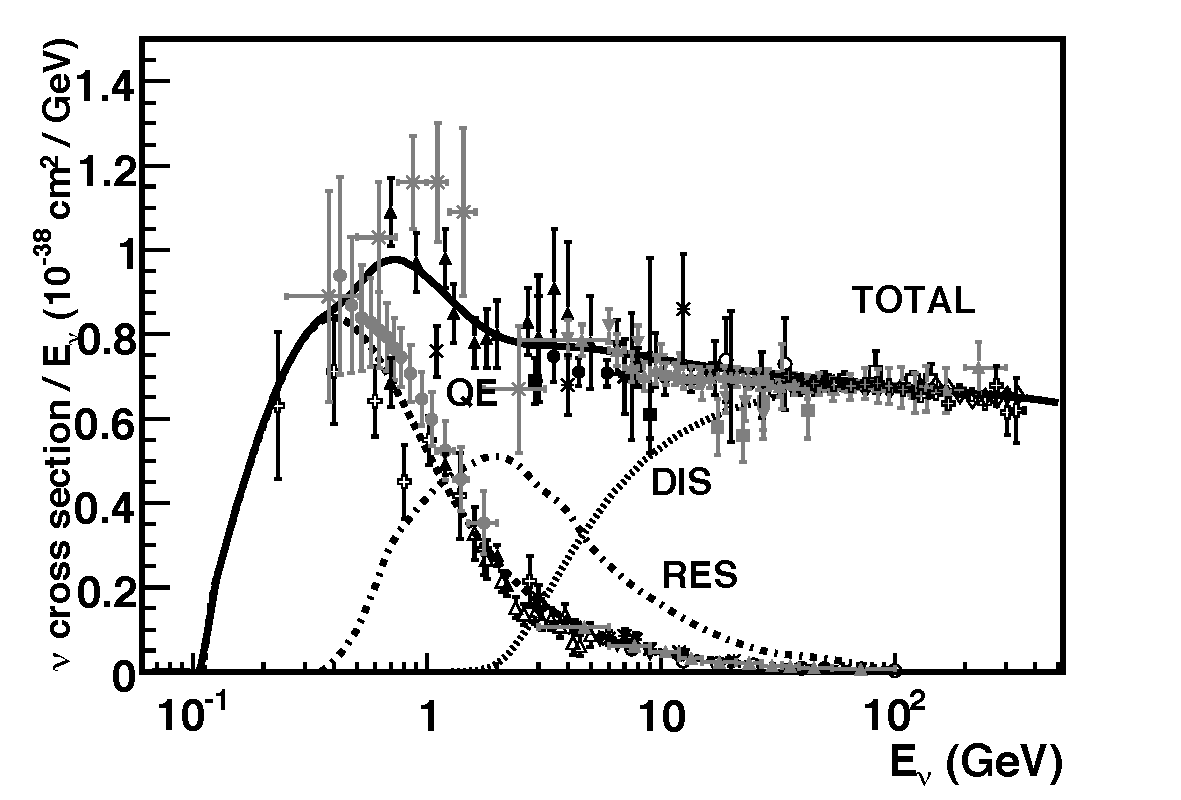
\includegraphics[width=\textwidth]{figures/theory/cc_inclusive_nu.pdf}
\caption{neutrinos}
\end{subfigure}
\begin{subfigure}[t]{0.45\linewidth}
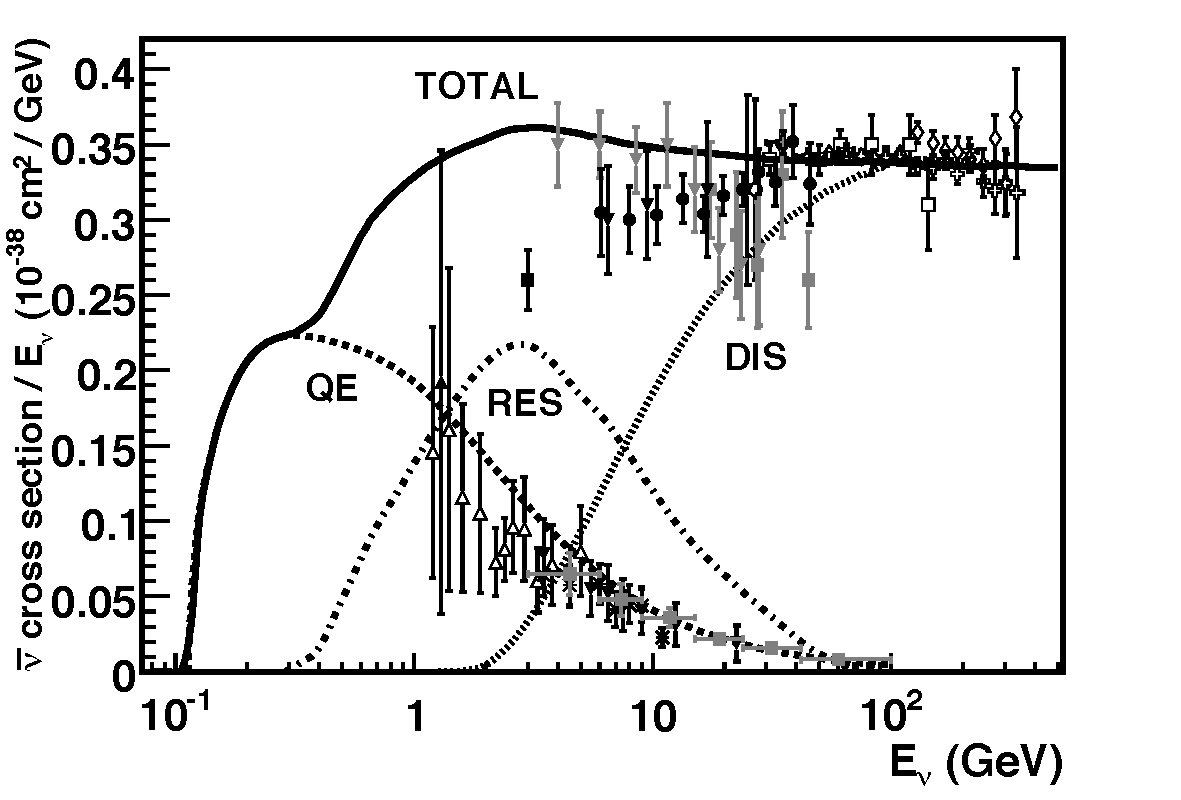
\includegraphics[width=\textwidth]{figures/theory/cc_inclusive_nubar.pdf}
\caption{antineutrinos}
\end{subfigure}
\caption{Inclusive cross sections for neutrinos and antineutrinos. Figure taken from \cite{Formaggio:2012aa}.}
\end{figure*}


